% 1way_coupling_prescribed_rotation.tex

\documentclass[11pt]{standalone}

\pagestyle{empty}

% load packages:
\usepackage{amsmath}
\usepackage{amssymb}
\usepackage{amstext}
\usepackage{amsfonts}
\usepackage{units}

% TikZ:
\usepackage{tikz}
\usetikzlibrary{shapes.geometric, arrows, intersections, through, decorations.text, decorations.shapes, backgrounds}

\usepackage{pgfplots}

% Use newest spacing options (from v. 1.3 on)
\pgfplotsset{compat=newest}
\pgfplotsset{width=10cm}
\pgfplotsset{height=6cm}

\pgfplotsset{grid style={solid}}

% Remove white space from generated pdf,
% thus otaining a pdf with only the picture that can
% easily be included in a(nother) tex-document via the usual \includegraphic command.
% Benefit: 1. you can keep your pictures organised in a subfolder and
%          2. the picture remains a vector graphic :)
%\usepackage[active, tightpage]{preview}
%\PreviewEnvironment{tikzpicture}
%\setlength\PreviewBorder{0pt}
% Alternatively, delete the three lines above and run 'pdfcrop filename.pdf',
% the result should be the same.

\begin{document}

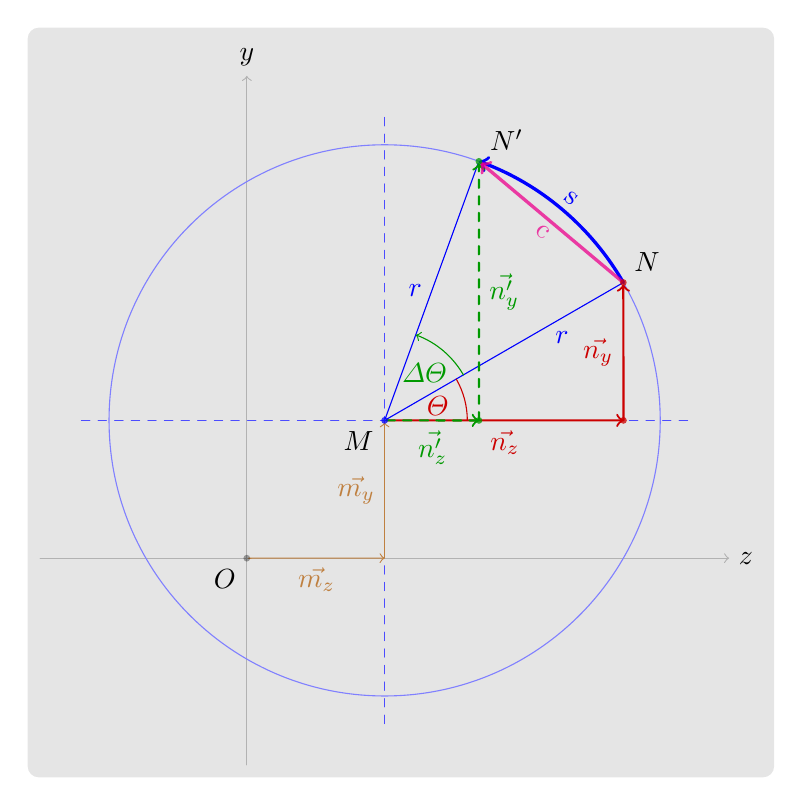
\begin{tikzpicture}[scale=3.5,cap=round,
                    show background rectangle,
                    background rectangle/.style={fill=gray!20, rounded corners}
                   ]
  % Local definitions
  \def\radius{1.0}
  \def\startangle{30}
  \def\endangle{70}

  % Colors
  \colorlet{ncolor}{red!80!black}
  \colorlet{newncolor}{green!60!black}
  \colorlet{radiuscolor}{blue}
  \colorlet{mcolor}{brown!100}

  % Styles
  \tikzstyle{axes}=[color=black!30]
  \tikzstyle{rot-axes}=[color=blue!70, dashed, thin]
  \tikzstyle{important line}=[very thick]
  \tikzstyle{information text}=[rounded corners,fill=red!10,inner sep=1ex]
  \tikzstyle{point}=[circle, inner sep=.0pt]


% Axes:
  \node[style=point, label=below left:$O$] (O) at (-0.5,-0.5) {};
  \draw[->, style=axes, name path=z-axis] (-1.25,-0.5) -- (1.25,-0.5) node[right, color=black] {$z$};
  \draw[->, style=axes, name path=y-axis] (-0.5,-1.25) -- (-0.5,1.25) node[above, color=black] {$y$};

% Centre of rotational axis:
  \node[style=point, label=below left:$M$] (M) at (0,0) {};
% Rotational axis:
  \draw[style=rot-axes, name path=rot-z-axis] (-1.1,0) -- (1.1,0) {};
  \draw[style=rot-axes, name path=rot-y-axis] (0,-1.1) -- (0,1.1) {};
% M-vectors:
  \draw[->, mcolor] (O) -- node[below] {$\vec{m_z}$} (0,-0.5);
  \draw[->, mcolor] (0,-0.5) -- node[left] {$\vec{m_y}$} (M);
%   \draw[->, mcolor] (O) -- node[left] {$\vec{m_y}$} (-0.5,0);
%   \draw[->, mcolor] (-0.5,0) -- node[above] {$\vec{m_z}$} (M);

% Rotation/Circle:
  \draw[name path=circle, color=blue!50] (M) circle (\radius);

% Node of solid mesh, that rotates:
  \node[style=point, label=above right:$N$] (N) at (\startangle:\radius) {};
  % Alternatively: use intersections:
%   \draw[name path=myline, color=blue, thick] (40:0.0cm) -- (40:1cm);
%   \fill[red,name intersections={of=circle and myline}]
%       (intersection-1) circle (1pt) node {1};

% Destination of N within dt seconds:
  \node[style=point, label=above right:$N'$] (N') at (\endangle:\radius) {};

% Arc that a node N travels in dt:
  \draw[->, important line, color=radiuscolor, postaction={decoration={text along path, text color=radiuscolor, text={s},text align={align=center}, reverse path, raise=3pt} ,decorate}] (N) arc(\startangle:\endangle:\radius);

% Draw connecting lines:
  \draw[name path=MN, radiuscolor] (M) -- node[below=-5pt, right=15pt] {$r$} (N);
  \draw[name path=MN', radiuscolor] (M) -- node[left] {$r$} (N') ;
%   \draw[name path=NN'] (N) -- node[below=1pt, left=1pt] {$c$} (N') ;

% Draw z and y vectors from M to N and N':
%   \draw (30:1cm) -- node[right=1pt,fill=red] (intersection of N--0.8,0 and z-axis) coordinate (d) {};
% \draw[style=important line] (N) -- node [right=1pt,fill=red]
%       {} (intersection of N--+(0,0) and 0,0--1,0) coordinate (t);

% Find points along z-axis:
  \path[name path=N--Z] (N) -- +(0,-1);
  \path[name intersections={of=N--Z and rot-z-axis, by=NZ}];
 \path[name path=N'--Z] (N') -- +(0,-1);
%   \path[name path=N'--Y] (N') -- +(-1,0);
 \path[name intersections={of=N'--Z and rot-z-axis, by=N'Z}];
%   \path[name intersections={of=N'--Y and rot-y-axis, by=N'Y}];
% And draw lines for y- and z-coordinates of the vectors from M to N and N':
  \draw[->, ncolor, thick] (M) -- node[below] {$\vec{n_z}$} (NZ);
  \draw[->, ncolor, thick] (NZ) -- node[left] {$\vec{n_y}$} (N);
  \draw[->, newncolor, thick, dashed] (M) -- node[below] {$\vec{n'_z}$} (N'Z);
  \draw[->, newncolor, thick, dashed] (N'Z) -- node[right] {$\vec{n'_y}$} (N');

% Angles:
  \node (NTheta) at (\startangle:0.3) {};
  \draw[ncolor] (0.3,0) arc(0:\startangle:0.3);
  \draw (\startangle*0.5:0.2) node[ncolor] {$\varTheta$};

  \node (N'Theta) at (\startangle:0.33) {};
  \node[newncolor] at (50:0.225) {$\varDelta\varTheta$};
  \draw[->,newncolor] (N'Theta) arc (\startangle:\endangle:0.33);

% Arrow for chord length:
%   \draw[->, black, thick] (N) -- node[below] {$\vec{m_y}$} (N');
  \draw[->, magenta, very thick, opacity=0.75, postaction={decoration={text along path, text color=magenta, text={c},text align={align=center}, reverse path, raise=-7pt} ,decorate}] (N) -- node[below left] {} (N');

% Points:
  \foreach \point in {M}
  \fill [blue, opacity=.75] (\point) circle (.35pt);
  \foreach \point in {O}
  \fill [black, opacity=.35] (\point) circle (.35pt);
  \foreach \point in {N, NZ}
  \fill [ncolor, opacity=.75] (\point) circle (.35pt);
  \foreach \point in {N', N'Z}
  \fill [newncolor, opacity=.75] (\point) circle (.35pt);

% Text:
%  \draw[xshift=30, yshift=30] node [right,text width=10cm,style=information text]
%    { The known Cartesian coordinates of the points $M$, and $N$ are
%      \[
%      { M = \begin{pmatrix} {\color{mcolor}m_y} \\ {\color{mcolor}m_z} \end{pmatrix}}, \; { N = \begin{pmatrix} n_1 \\ n_2 \end{pmatrix} = \begin{pmatrix} {\color{mcolor}m_y} + {\color{ncolor}n_y} \\ {\color{mcolor}m_z} + {\color{ncolor}n_z} \end{pmatrix}}
%      \]
%      in which $M$ is the center of rotation and $N$ a node of the mesh representing the turbine blades.
%%       \[
%%       { N' = \begin{pmatrix} n'_1 \\ n'_2 \end{pmatrix} = \color{newncolor}\begin{pmatrix} m_y+n'_y \\ m_z+n'_z \end{pmatrix}}
%%       \]
%      Given a number of rotations per minute, e.g.~$\text{rpm}=\unit[10]{min^{-1}}$, the angular velocity $\omega$ and displacement {\color{newncolor}$\varDelta\varTheta$} are computed by
%      \[ { \omega = 2\pi\cdot \text{rpm} }, \;\;\;\;
%         {\color{newncolor} \varDelta\varTheta } = \omega \varDelta t \]
%    };
%
%  \draw[xshift=40, yshift=-30] node [right,text width=10cm,style=information text]
%    {
%      Within $\varDelta t$ seconds, a node $N$ moves with an angular velocity $\omega$ along a circular arc {\color{radiuscolor}$s$} to it's position in $N'$.
%      To compute the coordinates of $N'$, we first compute the radius {\color{radiuscolor}$r$} and current angle {\color{ncolor}$\varTheta$} in the polar coordinate system.
%      \[ {\color{radiuscolor} r} = \sqrt{{\color{ncolor}n_y}^2 + {\color{ncolor}n_z}^2}, \;\;\;\;
%         {\color{ncolor} \varTheta} = \arcsin\left({\frac{{\color{ncolor}n_y}}{{\color{radiuscolor}r}}}\right). \]
%      Via simple trigonometrical functions we can then derive the coordinates of the destination $N'$.
%      \[ {\color{newncolor} n_y' } = {\color{radiuscolor} r } \cdot \sin\left( {\color{ncolor} \varTheta} + {\color{newncolor} \varDelta\varTheta} \right), \;\;\;\;
%         {\color{newncolor} n_z' } = {\color{radiuscolor} r } \cdot \cos\left( {\color{ncolor} \varTheta} + {\color{newncolor} \varDelta\varTheta} \right) \]
%      Thus the coordinates of $N'$ in the Cartesian coordinate system are
%      \[ { N' = \begin{pmatrix} n'_1 \\ n'_2 \end{pmatrix} = \begin{pmatrix} {\color{mcolor}m_y} + {\color{newncolor}n'_y} \\ {\color{mcolor}m_z} + {\color{newncolor}n'_z} \end{pmatrix}} \]
%    };

\end{tikzpicture}

\end{document}
